\documentclass[xcolor=svgnames,aspectratio=169]{beamer}
\usetheme{Boadilla}

\usepackage[utf8]{inputenc}
\usepackage[T1]{fontenc}
\usepackage{lmodern}
\usepackage{sourcecodepro}
\usepackage[whole]{bxcjkjatype}
\usepackage[backend=biber]{biblatex}
\addbibresource{octave.bib}
\usepackage{listings}
\lstset{
  language=Octave,
  basicstyle=\tiny,
  keywordstyle=\color{blue},
  morekeywords={classdef,endclassdef,properties,endproperties,methods,endmethods},
}
\usepackage{mathtools}
\usepackage{multimedia}
\usepackage{siunitx}
\usepackage{pifont}
\usepackage{tikz}
\newcommand*\colorcheck[1]{%
  \expandafter\newcommand\csname #1check\endcsname{\textcolor{#1}{\ding{52}}}%
}
\colorcheck{green}

\title[GNU Octave]{Your own GNU Octave under the Xmas tree
  
\includegraphics[width=1.5em]{res/images/octave-logo-1024.png}
}
\subtitle{Finish your numerical experiments before New Year's Eve}
\author[Kai T. Ohlhus]{
  オールフス カイトーベン \\
  OHLHUS, Kai Torben}
\institute[TWCU]{
  Graduate School of Science \\
  Tokyo Woman's Christian University}
\date[December 24, 2019]{JSIAM 11th Three-Group Meeting "Applied Mathematical Seminar" \\
at the University of Tokyo \\[1em]
December 24, 2019}
\titlegraphic{
\vfill
\hfill
\includegraphics[height=1em]{res/images/cc-by-sa}
}

\begin{document}

{
\usebackgroundtemplate{
  \vbox to \paperheight{\vfil\hbox to \paperwidth{\hfil
  \tikz\node[opacity=0.15] {
  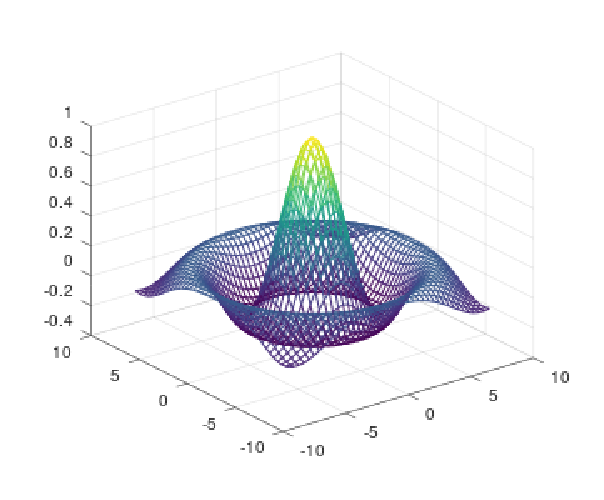
\includegraphics[width=0.6\paperwidth]{res/images/example-mesh}
  };
  \hfil}\vfil}
}
\frame{\titlepage}
}


\section{Setup for this meeting}
\frame{\tableofcontents}
\begin{frame}{Installing GNU Octave on other systems}
$\rightarrow$ \url{https://wiki.octave.org/Installation}
\bigskip
\begin{columns}
\begin{column}{0.4\textwidth}
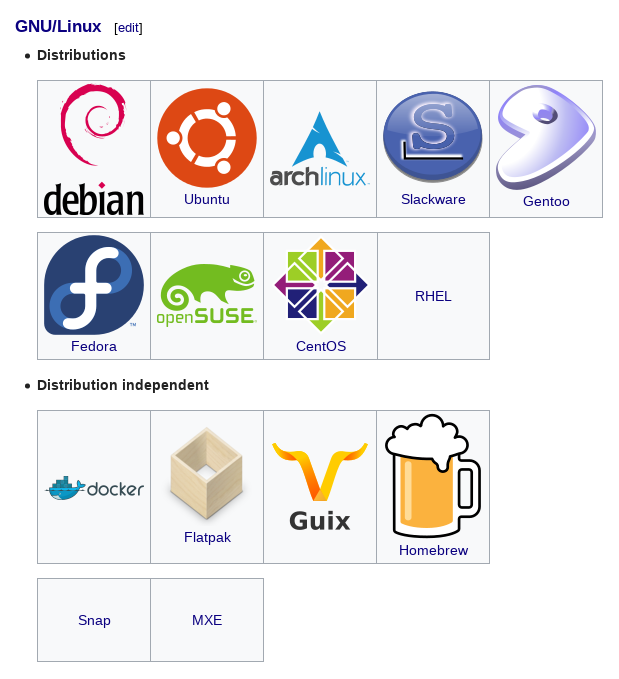
\includegraphics[width=\textwidth]{res/images/octave_wiki_install_linux}
\end{column}
\begin{column}{0.4\textwidth}
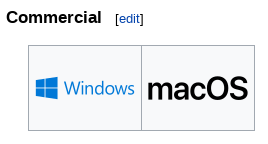
\includegraphics[width=0.42\textwidth]{res/images/octave_wiki_install_commercial}

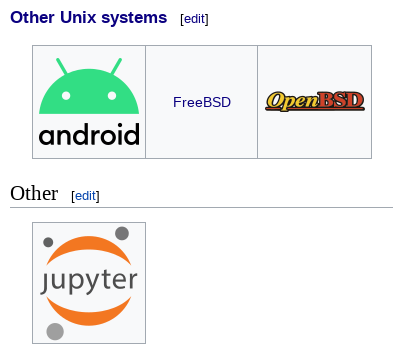
\includegraphics[width=0.6\textwidth]{res/images/octave_wiki_install_other}
\bigskip\bigskip\bigskip
\end{column}
\end{columns}

\end{frame}


\section{About GNU Octave}
\frame{\tableofcontents[currentsection]}
\begin{frame}{What is GNU Octave? - A community perspective.}
\begin{center}
\includegraphics[width=0.8\textwidth]{res/libreoffice/octave_community}
\end{center}
\end{frame}



\begin{frame}{What is GNU Octave? - A technical perspective.}
\vspace*{-1em}
\begin{center}
\includegraphics[width=0.8\textwidth]{res/libreoffice/octave_structure}
\end{center}
\end{frame}



\begin{frame}{Why GNU \textbf{"Octave"}?}

\begin{itemize}
\itemsep2em
\item
About \textbf{1992} \textbf{\color{DarkBlue}John W. Eaton (jwe)}
starts development\\[0.5em]
\begin{itemize}
\itemsep1em
\item
since then in total about \textbf{440 contributors}
\item
currently about \textbf{10-14 active developers}\footnote{Contributions to Octave core within last (two) month(s). \\
$\quad$ \texttt{\tiny hg log -r"date('>2019-11-24')" | grep user | sort | uniq}}
\end{itemize}

\item
Named after \textbf{\color{DarkBlue}Octave Levenspiel} (1926-2017)\\[0.5em]
\begin{itemize}
\itemsep1em
\item
former professor of jwe
\item
famous for quick back-of-the-envelope calculations
\end{itemize}
\end{itemize}
\end{frame}


\begin{frame}{Why \textbf{"GNU"} Octave?}

\begin{itemize}
\itemsep1.5em
\item
"GNU" (recursive: "GNU's Not Unix!")
Octave since \textbf{1997} (version 2.0.6)

\item
Shared
\textbf{philosophy}\footnote{\url{https://www.gnu.org/philosophy/free-sw.html}}
with the \textit{GNU project}
(\textit{Free Software Foundation}, FSF):\\[0.5em]

\begin{itemize}
\itemsep1em
\item
"[...] the freedom to run, copy, distribute, study, change
and improve the software. [...]"
\item
"[...] 'free' as in 'free speech,' not as in 'free beer'. [...]"

\end{itemize}

\item
Using \textbf{infrastructure} (e.g. code hosting and bug tracking)\\[0.5em]

\begin{itemize}
\item
SourceForge (1999), GitHub (2008), ...
\end{itemize}

\item
\textbf{Sponsorship} "Working Together for Free Software Fund"
\end{itemize}
\end{frame}



\section{"Hands on" session 1}
\frame{\tableofcontents[currentsection]}
\begin{frame}{"Hands on" session 1}
\begin{itemize}
\itemsep2em
\item
\textbf{\color{DarkBlue}\texttt{data\_io\_visualization.ipynb}}
\begin{itemize}
\item
Data I/O
\item
Plotting
\end{itemize}

\item
\textbf{\color{DarkBlue}\texttt{optimizing\_m\_code.ipynb}}

\item
\textbf{\color{DarkBlue}\texttt{fortran.ipynb}}
\begin{itemize}
\item
Octave and C/C++/Fortran
\end{itemize}

\item
In the GUI
\begin{itemize}
\item
Debugging and Profiling
\end{itemize}
\end{itemize}
\end{frame}



\section{Advanced Octave usage}
\frame{\tableofcontents[currentsection]}
\begin{frame}{Advanced Octave usage - Classes (1/3)}
\begin{columns}
\begin{column}[t]{0.2\textwidth}
\includegraphics[width=\textwidth]{res/libreoffice/octave_c_cpp_fortran_1}
\end{column}
\begin{column}{0.2\textwidth}
\ttfamily\scriptsize
\colorbox{green!30}{nice-package} \\
├ \colorbox{orange!30}{doc} \\
│ └─ \textbf{html-files} \\
├ \colorbox{orange!30}{inst} \\
│ ├─ \colorbox{orange!30}{private} \\
│ │ \ \ └─ \textbf{m-files} \\
│ └─ \textbf{m-files} \\
├ \colorbox{orange!30}{src} \\
│ ├─ C/C++-files \\
│ ├─ configure \\
│ └─ Makefile \\
├ CITATION \\
├ {\color{red!50!black}COPYING}  \\
├ {\color{red!50!black}DESCRIPTION} \\
├ INDEX    \\
├ Makefile \\
├ NEWS     \\
├ PKG\_ADD \\
└ PKG\_DEL \\
\end{column}
\begin{column}{0.5\textwidth}
\color{green!50!black}\scriptsize
package name \\[2em]
manual for the package \\[8em]
called if present \\
called by '\texttt{make}' if present \\
called by '\texttt{citation ("nice-package")}' \\
{\color{red!50!black}required} license \\
{\color{red!50!black}required} \\[1em]
for maintenance \\
list of code changes/improvements \\
commands run, when added   to   users path \\
commands run, when removed from users path
\end{column}
\end{columns}
\end{frame}
\begin{frame}{Advanced Octave usage - Packages (1/3)}
\begin{columns}
\begin{column}[t]{0.2\textwidth}
\includegraphics[width=\textwidth]{res/libreoffice/octave_c_cpp_fortran_1}
\end{column}
\begin{column}{0.2\textwidth}
\ttfamily\scriptsize
\colorbox{green!30}{nice-package} \\
├ \colorbox{orange!30}{doc} \\
│ └─ \textbf{html-files} \\
├ \colorbox{orange!30}{inst} \\
│ ├─ \colorbox{orange!30}{private} \\
│ │ \ \ └─ \textbf{m-files} \\
│ └─ \textbf{m-files} \\
├ \colorbox{orange!30}{src} \\
│ ├─ C/C++-files \\
│ ├─ configure \\
│ └─ Makefile \\
├ CITATION \\
├ {\color{red!50!black}COPYING}  \\
├ {\color{red!50!black}DESCRIPTION} \\
├ INDEX    \\
├ Makefile \\
├ NEWS     \\
├ PKG\_ADD \\
└ PKG\_DEL \\
\end{column}
\begin{column}{0.5\textwidth}
\color{green!50!black}\scriptsize
package name \\[2em]
manual for the package \\[8em]
called if present \\
called by '\texttt{make}' if present \\
called by '\texttt{citation ("nice-package")}' \\
{\color{red!50!black}required} license \\
{\color{red!50!black}required} \\[1em]
for maintenance \\
list of code changes/improvements \\
commands run, when added   to   users path \\
commands run, when removed from users path
\end{column}
\end{columns}
\end{frame}


\begin{frame}{Advanced Octave usage - Packages (2/3)}
\begin{columns}
\begin{column}[t]{0.2\textwidth}
\includegraphics[width=\textwidth]{res/libreoffice/octave_c_cpp_fortran_1}
\end{column}
\begin{column}{0.2\textwidth}
\ttfamily\scriptsize
\colorbox{green!30}{nice-package} \\
├ \colorbox{orange!30}{doc} \\
│ └─ \textbf{html-files} \\
├ \colorbox{orange!30}{inst} \\
│ ├─ \colorbox{orange!30}{private} \\
│ │ \ \ └─ \textbf{m-files} \\
│ └─ \textbf{m-files} \\
├ \colorbox{orange!30}{src} \\
│ ├─ C/C++-files \\
│ ├─ configure \\
│ └─ Makefile \\
├ CITATION \\
├ {\color{red!50!black}COPYING}  \\
├ {\color{red!50!black}DESCRIPTION} \\
├ INDEX    \\
├ Makefile \\
├ NEWS     \\
├ PKG\_ADD \\
└ PKG\_DEL \\
\end{column}
\begin{column}{0.5\textwidth}
\ttfamily\tiny
\colorbox{red!30}{DESCRIPTION} \\[0.5em]
Name: nice-package \\
Version: 1.0.0 \\
Date: 2019-12-24 \\
Author: First <first@home.net>, Second <first@home.net> \\
Maintainer: First <first@home.net>, Second <first@home.net> \\
Title: Some very nice package \\
Description: A short description of the package.  If this \\
\ description gets too long for one line it can continue \\
\ on the next by adding a space to the beginning of the \\
\ following lines. \\
License: GPLv3+ \\
{\color{red!50!black}Depends: package (>= 1.0.0)} \\
BuildRequires: libopenblas-dev [Ubuntu] openblas-devel \\[2em]

\colorbox{red!30}{INDEX} \\[0.5em]
\# A comment \\
nice-package >$ $> Some very nice package \\
Category Name 1 \\
 function1 function2 function3 \\
 function4 \\
Category Name 2 \\
 function2 function5 \\
\end{column}
\end{columns}
\end{frame}


\begin{frame}{Advanced Octave usage - Packages (3/3)}
\begin{columns}
\begin{column}[t]{0.2\textwidth}
\includegraphics[width=\textwidth]{res/libreoffice/octave_c_cpp_fortran_1}
\end{column}
\begin{column}{0.75\textwidth}
\small
Why all the effort?
\begin{itemize}
\itemsep1em
\item
Grouping of related code.

\item
Users can easily install your package from an \textbf{arbitrary URL}:

\texttt{\footnotesize pkg install https://www.url.org/nice-package-v1.0.0.tar.gz}

\begin{figure}

\includegraphics[width=4em]{res/images/octave-flower}
\end{figure}

\item
Upload to the \textbf{Octave Forge} \url{https://octave.sourceforge.io/}.
Package will be reviewed and can be easier installed via:

\texttt{\footnotesize pkg install {\color{red!50!black}-forge} nice-package}

\end{itemize}
\end{column}
\end{columns}
\end{frame}

\begin{frame}{Advanced Octave usage (summary)}
\begin{columns}
\begin{column}{0.15\textwidth}
\includegraphics[width=\textwidth]{res/libreoffice/octave_c_cpp_fortran_1}
\end{column}
\begin{column}{0.15\textwidth}
\includegraphics[width=\textwidth]{res/libreoffice/octave_c_cpp_fortran_2}
\end{column}
\begin{column}{0.3\textwidth}
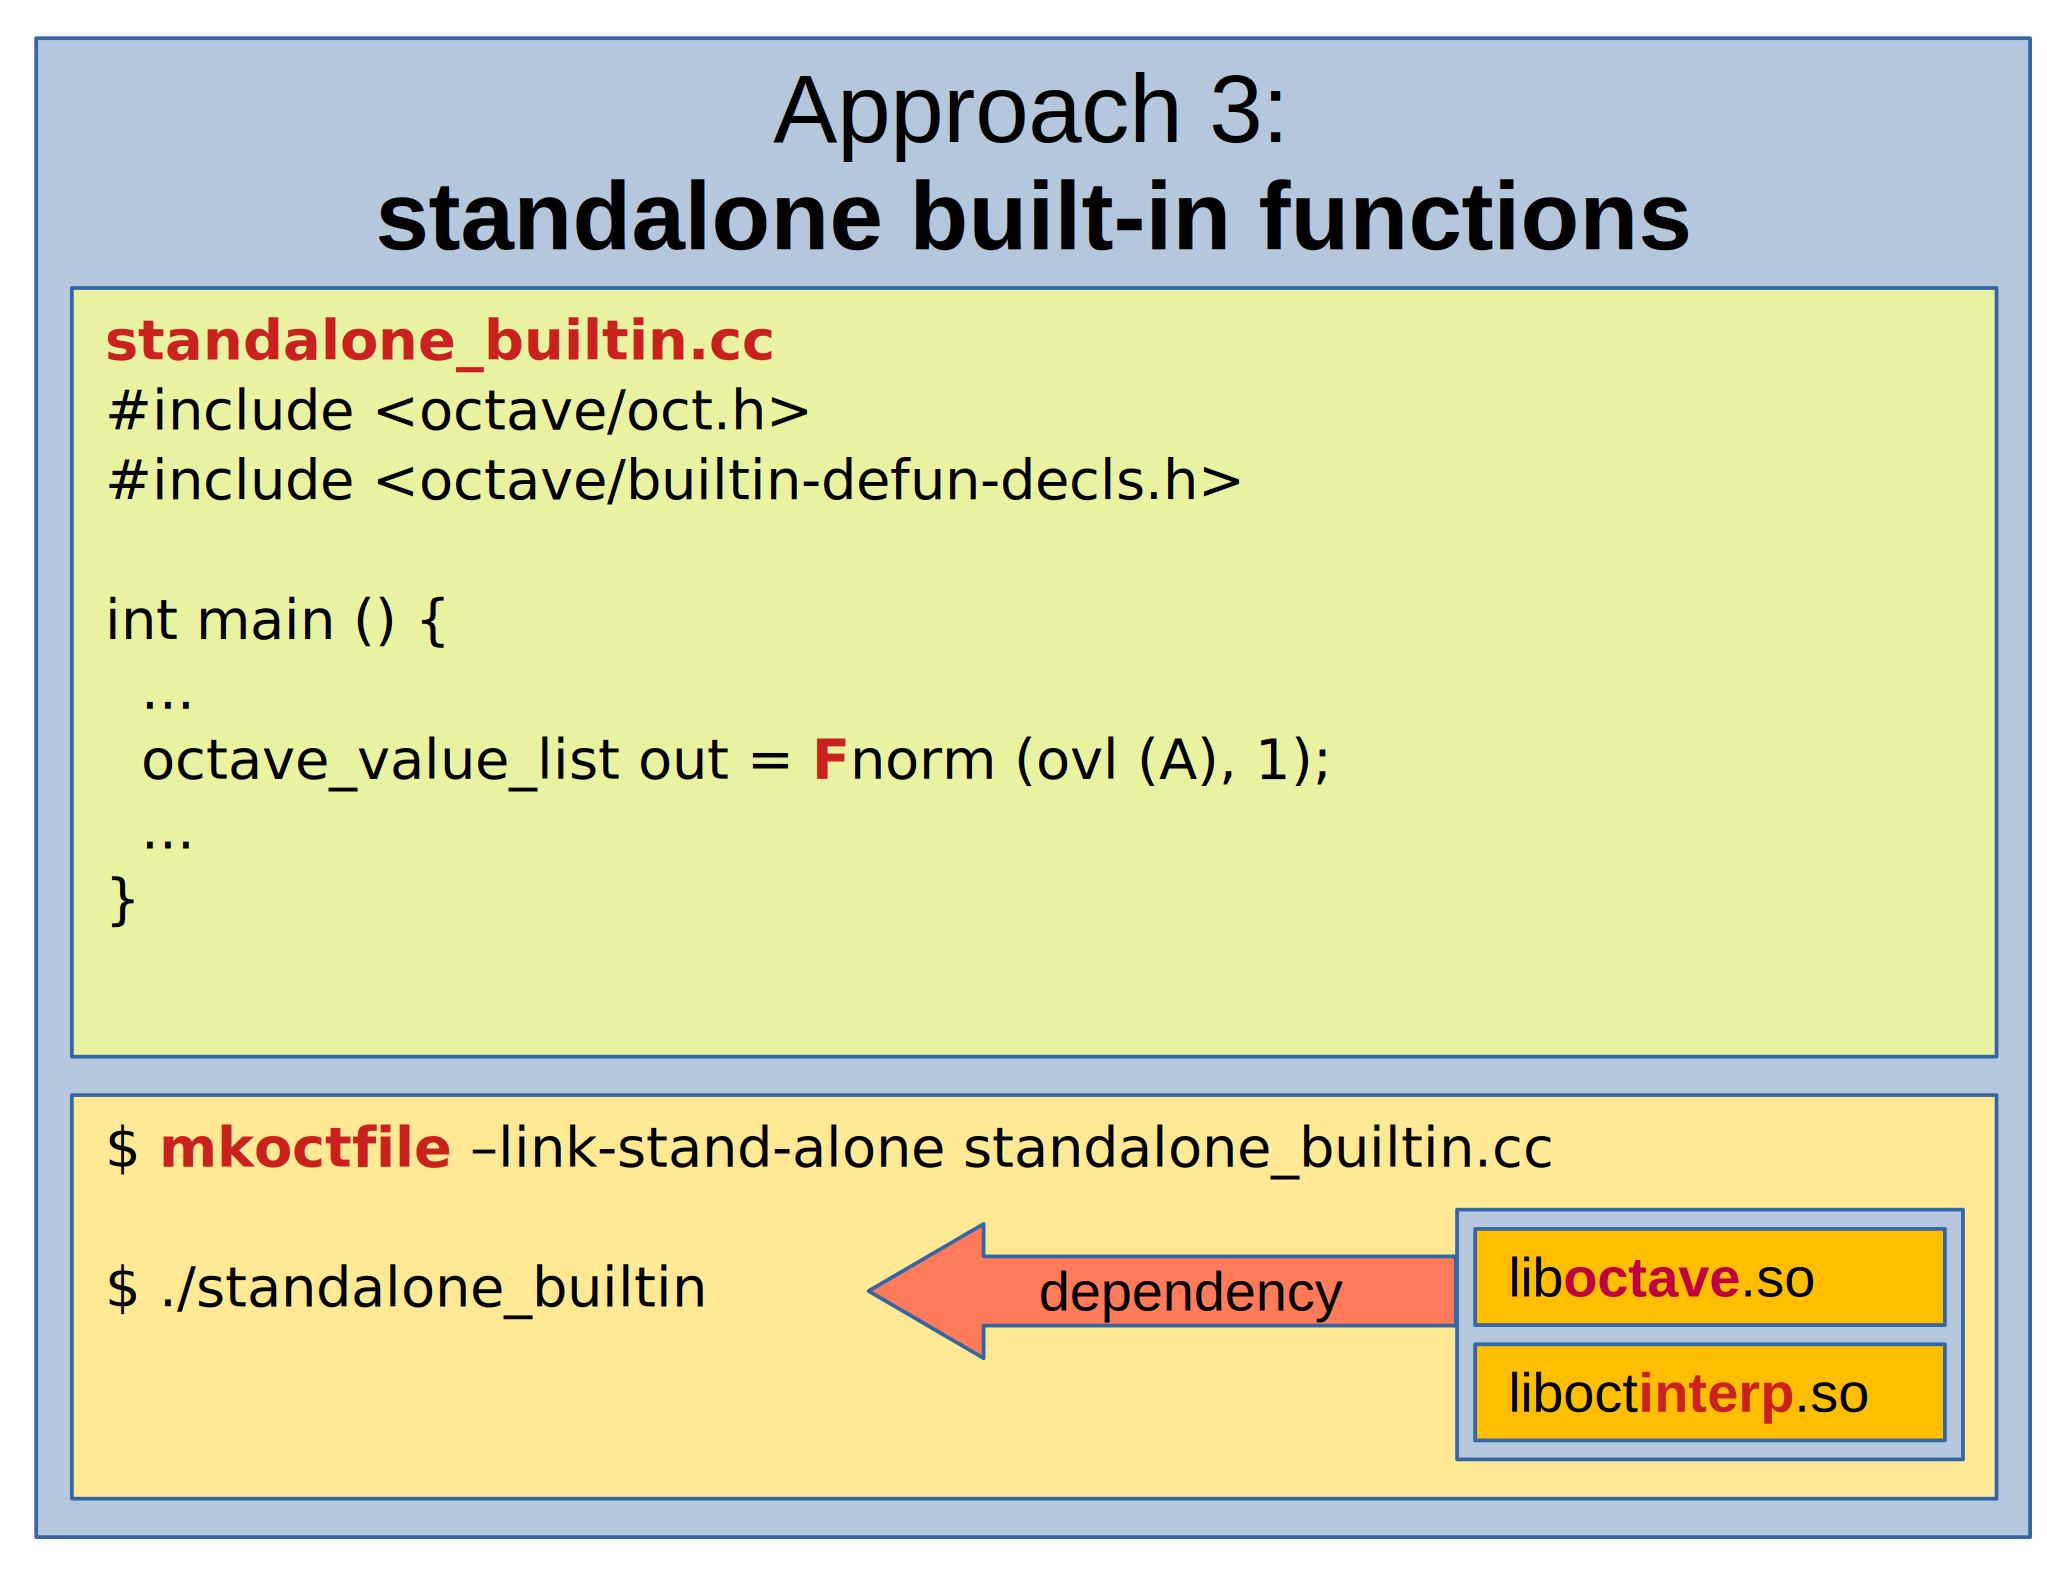
\includegraphics[width=\textwidth]{res/libreoffice/octave_c_cpp_fortran_3}
\end{column}
\begin{column}{0.3\textwidth}
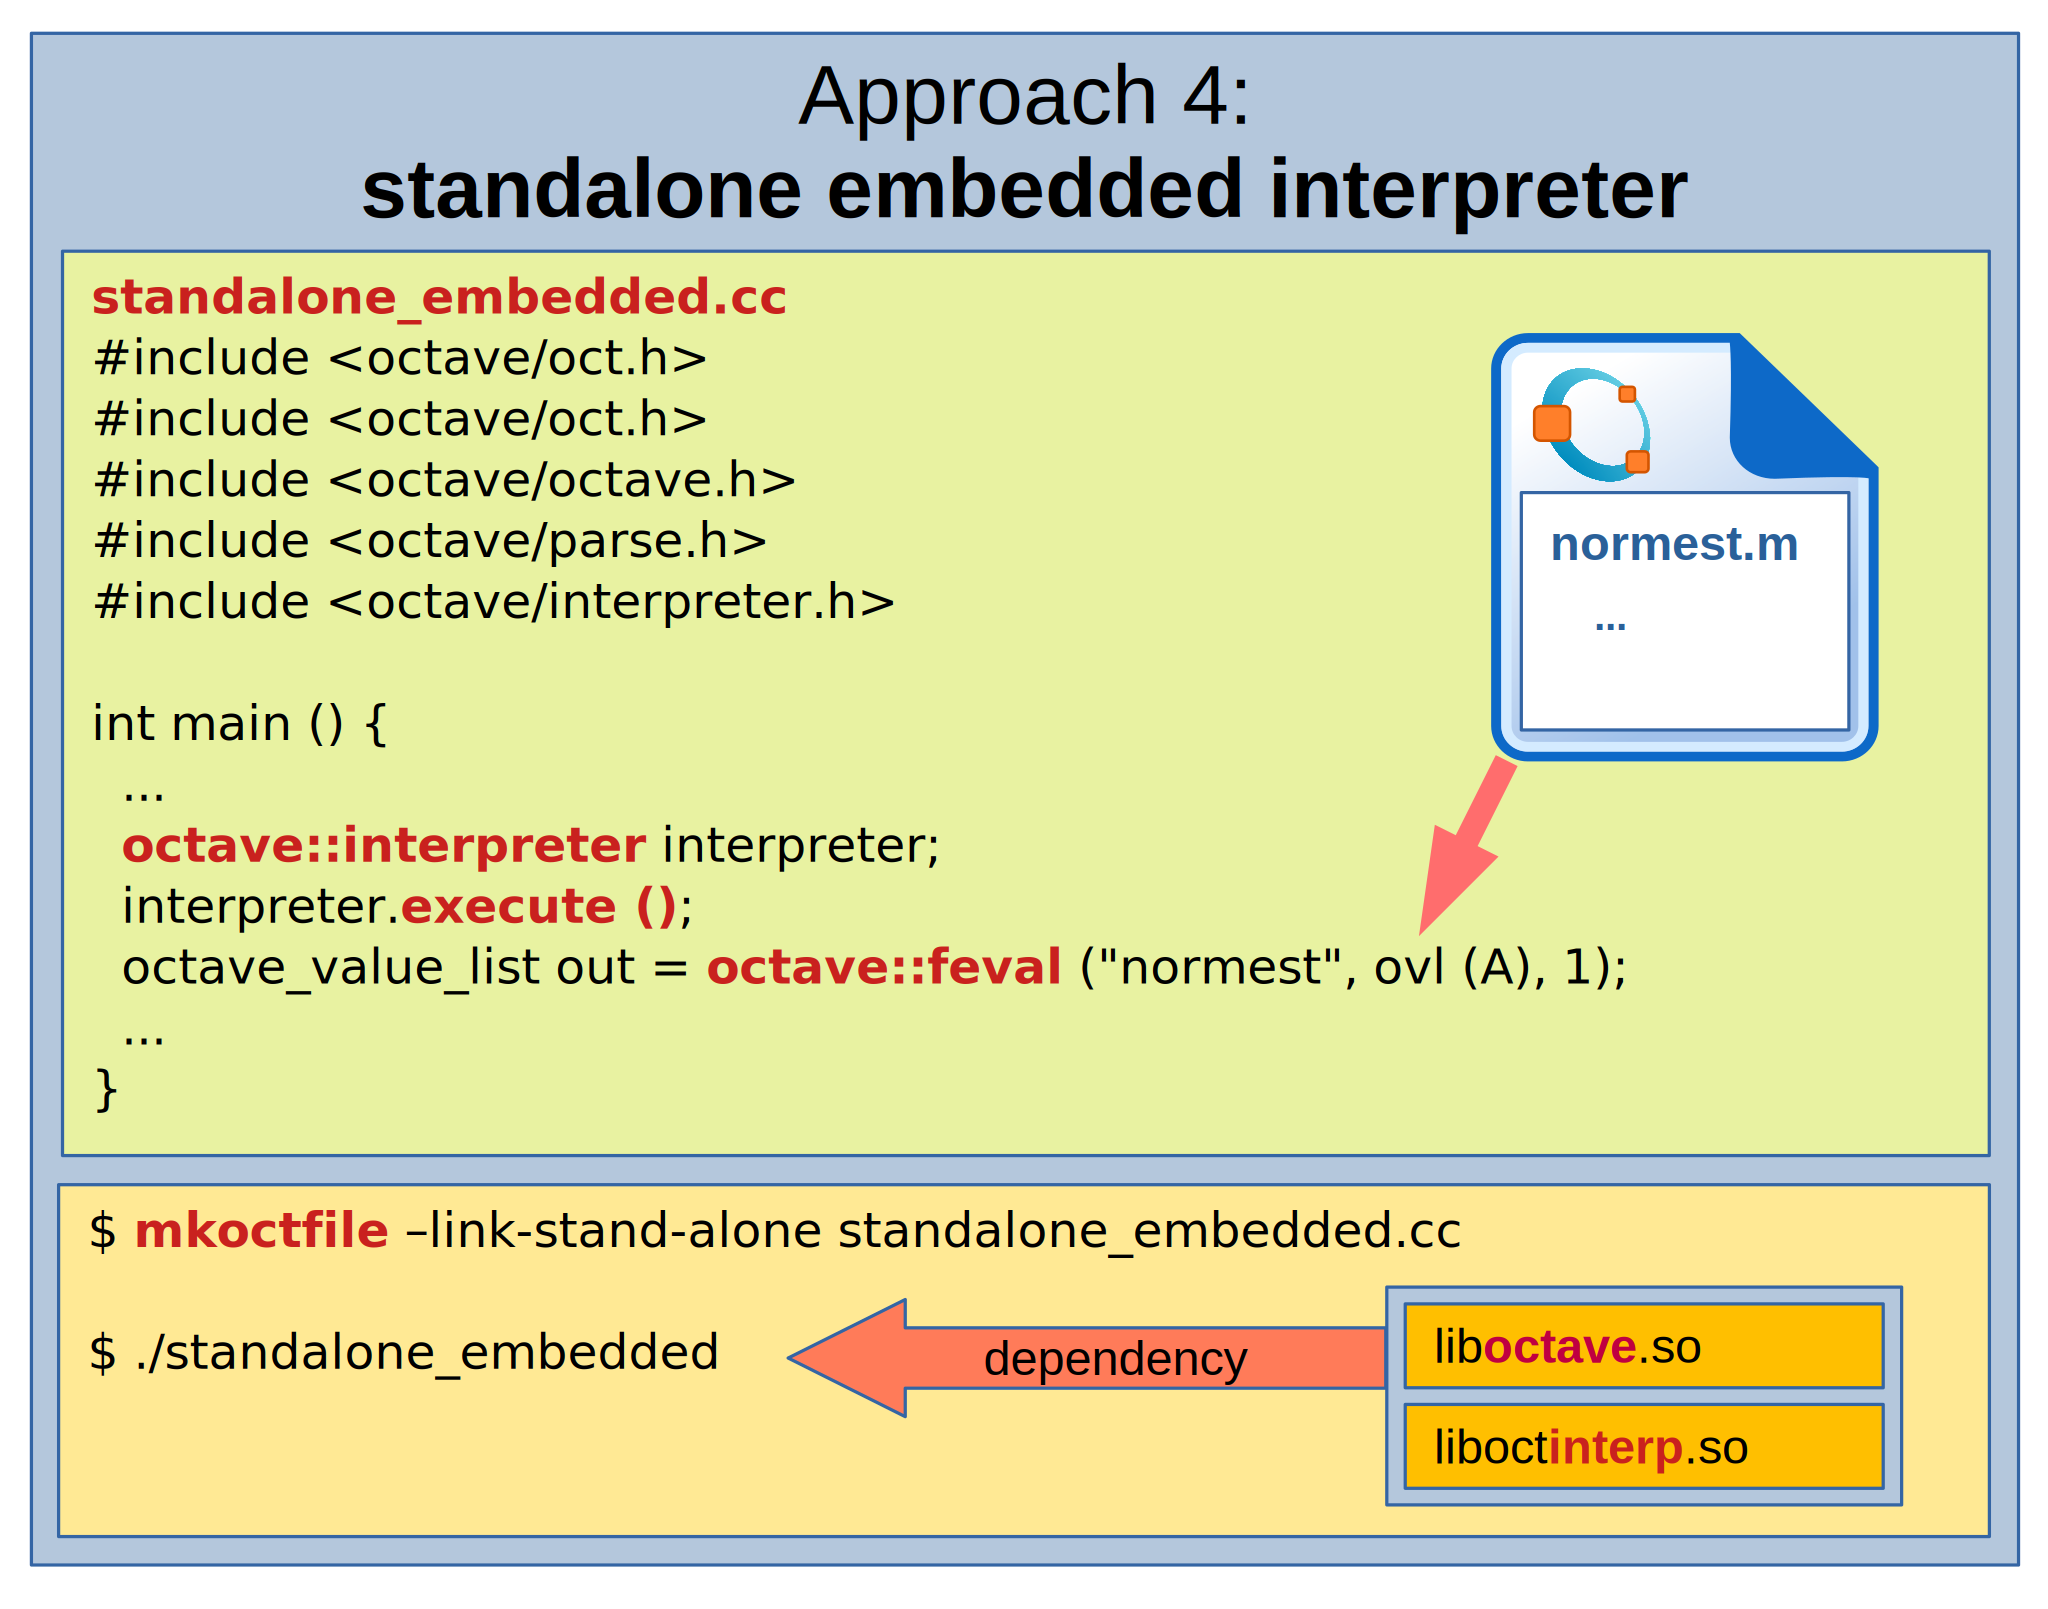
\includegraphics[width=\textwidth]{res/libreoffice/octave_c_cpp_fortran_4}
\end{column}
\end{columns}
easy \hfill difficult
\end{frame}


\section{"Hands on" session 2}
\frame{\tableofcontents[currentsection]}
\begin{frame}{"Hands on" session 2}
\begin{itemize}
\itemsep5em
\item
\textbf{\color{DarkBlue}\texttt{fortran.ipynb}}

\item
\textbf{\color{DarkBlue}\texttt{standalone.ipynb}}
\end{itemize}
\end{frame}



\section{Developing your own Octave}
\frame{\tableofcontents[currentsection]}
\begin{frame}{Octave development in a Nutshell}
\begin{center}
\includegraphics[width=0.85\textwidth]{res/libreoffice/dev_workflow}
\end{center}
\end{frame}


\begin{frame}
\begin{center}
\includegraphics[width=0.85\textwidth]{res/libreoffice/dirs_doc}
\end{center}
\end{frame}



\begin{frame}
\begin{center}
\includegraphics[width=0.85\textwidth]{res/libreoffice/dirs_examples}
\end{center}
\end{frame}


\begin{frame}
\begin{center}
\includegraphics[width=0.85\textwidth]{res/libreoffice/dirs_libgui}
\end{center}
\end{frame}


\begin{frame}
\begin{center}
\includegraphics[width=0.85\textwidth]{res/libreoffice/dirs_libinterp_liboctave_1}
\end{center}
\end{frame}


\begin{frame}
\begin{center}
\includegraphics[width=0.85\textwidth]{res/libreoffice/dirs_libinterp_liboctave_2}
\end{center}
\end{frame}


\begin{frame}
\begin{center}
\includegraphics[width=0.85\textwidth]{res/libreoffice/dirs_libinterp_liboctave_3}
\end{center}
\end{frame}


\begin{frame}{Some selected ongoing efforts}
From mailing-lists
and {\color{DarkBlue}\url{https://wiki.octave.org/Projects}}:\\[1em]
\begin{itemize}
\itemsep1em
\item
Octave.app for macOS
\hfill{\scriptsize\color{DarkBlue} \url{https://octave-app.org}}
\item
Python interface
\hfill{\scriptsize\color{DarkBlue} \url{https://wiki.octave.org/Pythonic}}
\item
Tabular data structure
\hfill{\scriptsize\color{DarkBlue}
\url{https://github.com/apjanke/octave-tablicious}}
\item
Improved \texttt{pkg} tool
\hfill{\scriptsize\color{DarkBlue}
\url{https://github.com/apjanke/octave-packajoozle}}
\item
Better graphics and \texttt{classdef} support
\item
Improved GUI terminal widget
\item
...
\end{itemize}
\end{frame}


\section{Reporting Bugs and Getting Help}
\frame{\tableofcontents[currentsection]}
\begin{frame}{Reporting problems, ask for help (1/2)}
Please, first look at:
\bigskip
\begin{itemize}
\item
\itemsep1em
{\color{DarkBlue}\url{https://octave.1599824.n4.nabble.com}}
(mailing-list archive)
\item
{\color{DarkBlue}\url{http://bugs.octave.org}} (bug tracker)
\end{itemize}
\bigskip\bigskip
\begin{columns}
\begin{column}{0.4\textwidth}
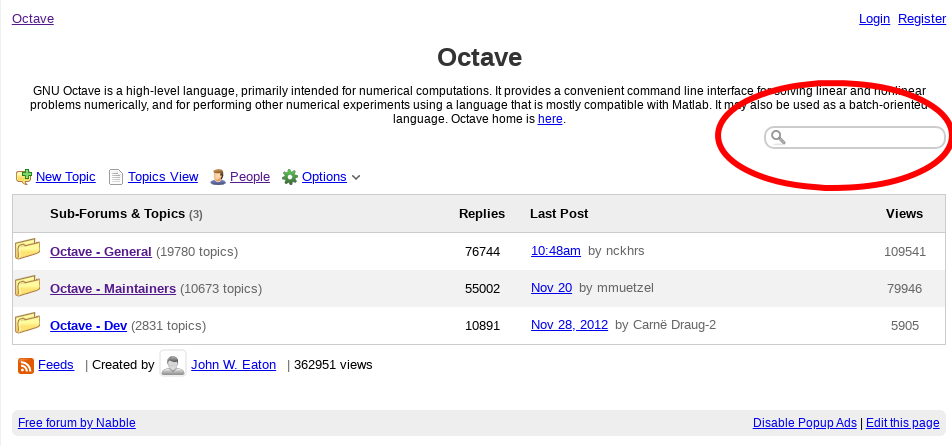
\includegraphics[width=\textwidth]{res/images/nabble_mailing_list_search}
\end{column}
\begin{column}{0.6\textwidth}
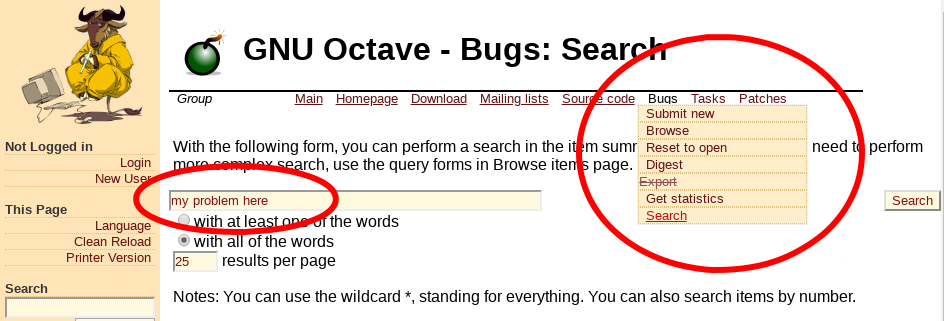
\includegraphics[width=\textwidth]{res/images/savannah_bug_search}
\end{column}
\end{columns}
\end{frame}



\begin{frame}{Reporting problems, ask for help (2/2)}
\begin{columns}
\begin{column}{0.55\textwidth}
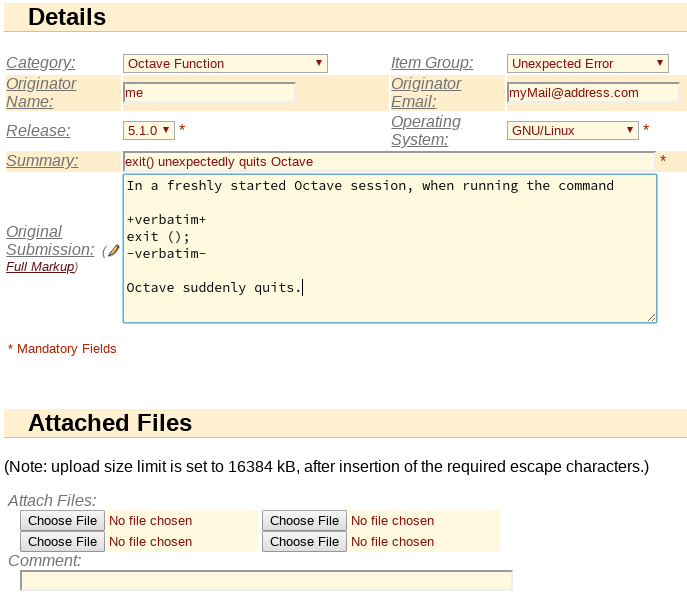
\includegraphics[width=0.9\textwidth]{res/images/savannah_bug_report}
\end{column}
\begin{column}{0.45\textwidth}
In case of any problems\\[0.8em]

\textbf{We are happy to help you!}\\[1em]
\begin{itemize}
\itemsep1em
\item
Write us:
\begin{itemize}
\itemsep1em
\item
{\color{DarkBlue}\url{help@octave.org}}
\item
IRC freenode (\#octave)
\end{itemize}
\item
Report us:
\begin{itemize}
\item
{\color{DarkBlue}\url{http://bugs.octave.org}}
\end{itemize}
\end{itemize}
\bigskip\bigskip
\end{column}
\end{columns}
\end{frame}



\section{Wrapping up}
\frame{\tableofcontents[currentsection]}
\begin{frame}{Wrapping up:}
\begin{itemize}
\itemsep2em
\item
What is GNU Octave?
\begin{itemize}
\itemsep1em
\item
High-level programming language, CLI/GUI software and community.

\item
A \textbf{convenient interactive interface}
for many well-known and well-performing
numerical, graphical and utility libraries
written in \textbf{C/C++, Fortran, Python, Java, ...} \\[0.8em]

Many possible (mis-)usage scenarios far beyond just opening a GUI window.

\item
\textbf{Free} to run, copy, distribute, study, change and improve.
\end{itemize}

\item
What it is \textbf{NOT}?
\begin{itemize}
\itemsep1em
\item
Not a \textbf{one-size-fits-all} solution for numerical computations.

\item
Not a compiled language, no transcompiler.

$\rightarrow$ There is an \textbf{interpreter overhead}.
\end{itemize}
\end{itemize}
\end{frame}



\begin{frame}
\begin{center}
\textbf{\Large Thank you for your attention!}
\bigskip

\includegraphics[width=0.5\textwidth]{res/libreoffice/octave_community}
\bigskip

\textbf{\Large Questions?}
\vfill\footnotesize
Slides and sources available at:
{\color{DarkBlue}\url{https://github.com/octave-de/octave_slides}}
\end{center}
\end{frame}


\end{document}
